\iffalse
\bibliography{myreference.bib}
\fi

%chapter 4
\chapter{Machine Learning Algorithm}
To figure out the importance of each feature in the feature vector, we use model-based methods to evaluate them. The statistics method such as pearson coefficient or chi-square can find the relationship between features and class, but since they are univariate feature methods, not considering the dependence between features, and the ultimate target is to train a model with better performance, it is reasonable to use models to directly tell us the feature importance. In this project, we use models with two representations, which is linear model and decision tree model.

\section{Logistic Regression}
It is a simple algorithm for training linear binary classifiers. Although its name contains ``regression'', it is a classification algorithm. It can be used when the input data is numeric type and nominal type. Numeric data means its value is continuous and its number is meaningful. Nominal data is consisted of several categories. If they are represented in number, the value is meaningless.

Linear model can be represented as the following equation:
\begin{equation} \label{Eq:linearModel}
z = \theta^Tx=\theta_0+\theta_1x_1+\theta_2x_2+...+\theta_nx_n
\end{equation}
where $x$ is the input vector. $n$ equals to the number of feature. $\theta$ is the coefficient of features. Then take this value into the \textit{sigmoid} function as:
\begin{equation} \label{Eq:sigmoidFunction}
h(z) = h_{\theta}(x) = \frac{1}{1+e^{-\theta^Tx}}
\end{equation}
The curve of sigmoid function is shown in Figure. \ref{fig:sigmoid}. In this figure, x-axis stands for the z we calculated in Eq. \ref{Eq:linearModel} and y-axis is $h(z)$. It is simply for doing a projection from $z$ to $h(z)$. Since logistic regression algorithm is used for training a binary classifier, we need a threshold to determine which input can be classified as 1 or 0. From this figure, we can see that if the value of z is larger than 0, then the value of $h(z)$ will be larger than 0.5. Thus, 0.5 is a suitable threshold. If $h(z)>0.5$ then the result is classified as 1, otherwise 0.
\begin{figure}[h]\centering
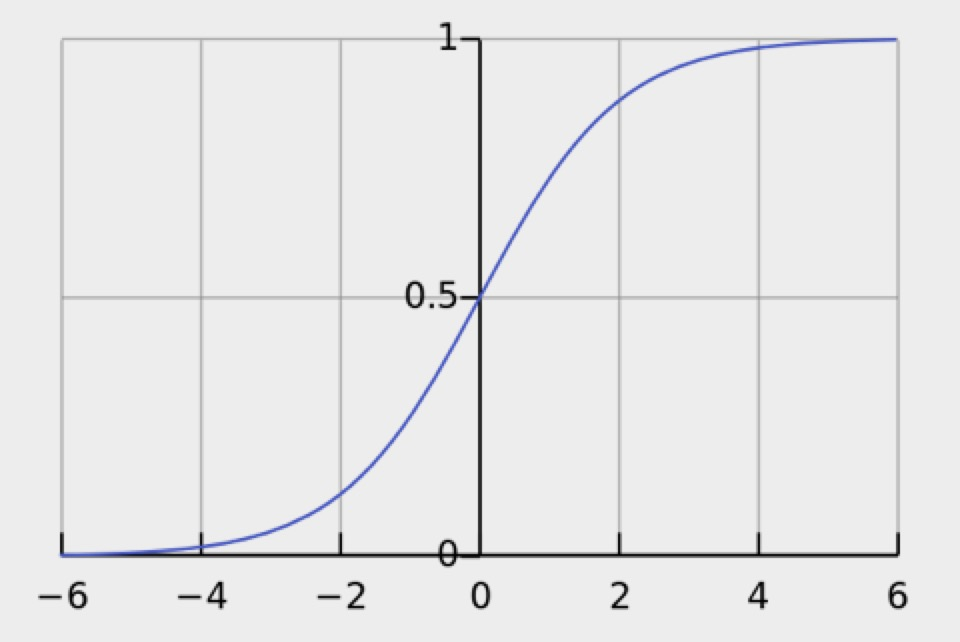
\includegraphics[width=0.9\textwidth]{sigmoid}
\caption{Curve of Sigmoid Function} \label{fig:sigmoid} \end{figure}

How to use this linear model to interpret the importance of features? The basic idea is using coefficients of the linear model $\theta$ in Eq. \ref{Eq:linearModel}. The most important features should have the highest coefficients in the model. If the feature is uncorrelated with the class, its coefficient value should close to zero. So how to train the coefficient $\theta$? In logistic regression, the idea is gradient descend.

First we need to define cost function $J$ of logistic regression in \ref{Eq:costFunction}
\begin{equation} \label{Eq:costFunction}
J(\theta)=\frac{1}{m}\sum_{i=1}^m{Cost(h_{\theta}(x^{(i)}),y^{(i)})}
\end{equation}
where m is the number of sample. $Cost(h_{\theta}(x^{(i)}),y^{(i)})$ is the error in each sample. It can be represented as Eq. \ref{Eq:costgroup}
\begin{equation} \label{Eq:costgroup}
Cost(h_{\theta}(x^{(i)}),y^{(i)})=
\left\{
\begin{array}{rcl}
-\log{(h_{\theta}(x^{(i)}))} & if \ y^{(i)} = 1\\
-\log{(1-h_{\theta}(x^{(i)}))} & if \ y^{(i)} = 0
\end{array}
\right.
\end{equation}

In Eq. \ref{Eq:cost}, if a sample is labeled as $y^{(i)}=1$, we want the cost of the model on this sample is 0, then $-\log{(h_{\theta}(x^{(i)}))}$ should be 0. Also, we know the classification result is $y_{classify}^{(i)}=1$ when the value of $h_{\theta}(x^{(i)}) > 0.5$. Thus the value of $-\log{(h_{\theta}(x^{(i)}))}$ is close to 0, which is what we want. The situation when $y^{(i)}=0$ is similar. So we can do a furtuer simplification into following equation. 
\begin{equation} \label{Eq:cost}
Cost(h_{\theta}(x^{(i)}),y^{(i)})=-y^{(i)}\log{(h_{\theta}(x^{(i)}))}-(1-y^{(i)})\log(1-h_{\theta}(x^{(i)}))
\end{equation}
It is equaled to Eq. \ref{Eq:costgroup}
Thus the cost function of logistic regression is:
\begin{equation} \label{Eq:newCostFunction}
J(\theta)=\frac{1}{m}[-y^{(i)}\log{(h_{\theta}(x^{(i)}))}-(1-y^{(i)})\log(1-h_{\theta}(x^{(i)}))]
\end{equation}
So far, we can use gradient descend to minimize $J(\theta)$. $\theta$ is an (D+1)-dimension vector if the input feature vector is D-dimension. The extra 1 dimension is the bias term for $x_0$ in Eq. \ref{Eq:linearModel}. To calculate the gredient, we need to calculate partial derivative with respect to each element in $\theta$ and minus it in Eq.
\begin{equation}
\label{Eq:thetaUpdate}
\theta_j := \theta_j - \alpha \frac{\partial}{\partial\theta_j}J(\theta)
\end{equation}
where j is the $j$-th coefficient and ``$:=$'' means update the value of $\theta_j$ using the formula on the right side. What is worth mentioning is that all the coefficient of feature in the vector should be updated simultaneously. $\alpha$ is the learning rate meaning how much distance $\theta$ wants to ``walk'' downward at each iteration. The value is preset by us. If it is too small, the learning procedure may take a long time. If it is too large, the value of $J(\theta)$ may even not convergent.

Interpreting the importance of feature by the value of coefficient is a feasible method. However, to make the result more accurate, we need to do further process.
\subsection{Reguralized Logistic Regression}
Overfitting\footnote{\url{https://en.wikipedia.org/wiki/Overfitting}} is a common concept in statistics and machine learning. It means that if our model learns too much from the training dataset, the overfitting may occur. To be more specific, if the model fit the data too well, the model may become more complex, which describes more noise instead of underlying relationship of data. In other word, if the model have too many feature, it will fails to generalize on new samples. To address overfitting, one of a popular method is \textit{regularization}.

If we don't want too many feature to make contribution on the model, we can simply set the coefficient of corresponding feature into 0. However, it is an NP-hard problem to solve because we have $2^N$ permutations and need to do searching for the best setting. To simplify this problem, we use Eq. \ref{Eg:regularizedConstraint} as an constriant to substitute the NP-hard problem.
\begin{equation} \label{Eg:regularizedConstraint}
\sum_{j=1}^D{\theta_j^2}\leq{C}
\end{equation}
How to solve this problem of minimizing $J(\theta)$ with a constraint condition? The answer is using the \textit{Lagrange Multiplier}\cite{bertsekas2014constrained}. We want to find a lagrange multiplier $\lambda>0$ and put the constraint condition into the minimization equation of $J(\theta)$ with the help of $\lambda$. Thus the Eq. \ref{Eq:newCostFunction} would be changed into the following equation:
\begin{equation} \label{regularizedCostFunction}
J(\theta)=-\frac{1}{m}\sum_{i=1}^m{[y^{(i)}\log{(h_{\theta}(x^{(i)}))}+(1-y^{(i)})\log(1-h_{\theta}(x^{(i)})) + \frac{\lambda}{2m}\sum_{j=1}^D{\theta_j^2}]}
\end{equation}
where $\sum_{j=1}^D{\theta_j^2}$ is named as \textit{regularizer}. Thus the Eq. \ref{Eq:thetaUpdate} becomes:
\begin{equation}
\label{thetaUpdateRegularized}
\theta_j := \theta_j - \alpha \frac{\partial}{\partial\theta_j}J(\theta)+\frac{\lambda}{m}\theta_j
\end{equation}
where j starts from 1 to D, not including the bias term. This regularization is call \textit{L2-norm} regularization. Another kind of regularization is called \textit{L1-norm} regularization. The difference between L1 and L2 is that in L1-norm regularization, the regularizer is $\sum_{j=1}^D{|\theta_j|}$. Using L1-norm regularization, the coefficient of weak feature will be 0. Thus, the feature vector may be sparse\cite{ng2004feature}.

\subsection{Multicollinearity of Features}
When there are multiple correlated features, the model trained by logistic regression will be unstable\cite{farrar1967multicollinearity}. It means that the coefficient would have a large change even if the value of data has a tiny change. For example, we have a dataset generated from a model $y=x_1+x_2$ and $x_1$ and $x_2$ are highly correlated such as $x_1\approx x_2$. We manually add some noise $\epsilon$. Then we take this noise-additive dataset into an algorithm. Ideally the trained model would be $y=x_1+x_2$. But it may be $y=2x_1$ or $y=-x_1+3x_2$ due to the noise. Thus, we need to do a filter-based feature selection to remove the correlation between features before training the model.

\subsubsection{Correlation-based Feature Selection}
Hall and Mark proposed a method called Correlation-based feature selection (CFS)\cite{hall1999correlation} in 1999. It is a special filter-based feature selection because it ranks a subset of feature rather than individual feature, which means that this method consider the dependence between features.

CFS algorithm is a heuristic for evaluating \textit{merit} of a subset of features. This heuristic is based on:

\textit{Good feature subsets contain features highly correlated with the class, yet uncorrelated with each other}\cite{hall2000textordfemininecorrelation}.

The heuristic can be formulized as:
\begin{equation} \label{Eq:merit}
Merit_s=\frac{k\overline{r_{cf}}}{\sqrt{k+k(k-1)\overline{r_{ff}}}}
\end{equation}
where $Merit_s$ is the heuristic ``merit'' of one subset of feature. $k$ is the number of feature in this subset. $\overline{r_{cf}}$ is the average feature-class correlation and $\overline{r_{ff}}$ is the average feature-feature intercorrelation. These two correlation can be calculated as Pearson's correlation coefficient or other coefficient. In Eq. \ref{Eq:merit}, the numerator indicates how predictive is this subset of feature while the denominator tells how much redundancy between them. By selecting the subset with large value of \textit{Merit}, this heuristic method can remove the subset composed of highly-correlated features and poor predictors of the class.

\subsection{Feature Scaling}
It is a simple but necessary problem needed to be solved when we use coefficient of feature to indicate the importance. If not, the model will be governed by the feature with large range of value.

\subsubsection{Normalization}
The general formula is:
\begin{equation} \label{normalization}
x'=\frac{x-x_{min}}{x_{max}-x_{min}}
\end{equation}
where $x_{min}$ and $x_{max}$ are the minimum and maximum value in the feature. After doing this processing, the range would be scaled into [0, 1].
\subsubsection{Standardization}
Feature standardization makes the value of each feature have zero-mean and unit-variance. It is widely used in many machine learning algorithm such as logistic regression and support vector machine. The general formula is:
\begin{equation} \label{standardization}
x'=\frac{x-\bar{x}}{\sigma}
\end{equation}
where $\bar{x}$ is the mean of the value of $x$ and $\sigma$ is its standard deviation.

After the three procedure above, the trained model can be used to indicate the importance of features. However, due to the CFS method, we can only input the feature without correlation. If we want to figure out all the importance of feature in the vector, we need to use other technique, such as the random forest that we will discuss in the next section.

\section{Random Forest}
Random Forest is a ensemble algorithm for classification. The model trained by this algorithm are represented as many decision trees, which is one of the popular algorithm\cite{safavian1991survey}. When we use the test set to evaluate this model, the output are determined by voting. For example, there are 5 trained decision tree in this forest. if the output y of one sample are classified as ``A'' by three trees and ``B'' by two trees, then the output is ``A''. If the comparison are even, just randomly choose one to be the output class.

To explain this method more convenient, we need to introduce the decision tree algorithm. A decision tree has internal node, branch and leaf. Each internal node is labeled with an input feature. Each leaf represents a value or class. The branch from a internal node are labeled with a specific requirement towards the feature on this node. If a node extends two branches, then the dataset on this node are separated into two parts according to the requirement on the branch.

How to choose the feature on each node and what requirement are needed to split the node? In decision tree, we use \textit{impurity decrease} as the metric. First we want to discuss the coefficient that can represent the \textit{impurity}.
\subsection{Impurity}
\subsubsection{Gini Index}
Gini index is a measure of statistical dispersion\cite{ceriani2012origins}. If the value is zero, means that all the values are the same. It can be calculated by:
\begin{equation} \label{Eq:Gini}
GINI(S) = 1-\sum_i{p_i}^2
\end{equation}
where $p_i$ is the fraction or probability of item labeled with $i$ in the dataset.
\subsubsection{Entropy}
Entropy is a numeric measure to quantify the concept of uncertainty. If the value of entropy is large, the uncertainty is higher. It has been discussed in chapter 2, with Eq. 2.2.
\subsection{Information Gain or Impurity Decrease}
We have discuss the concept of mutual information in chapter 2. Actually, the information gain is the same as the mutual information from the equation. It expresses the impurity decrease if we know a condition, which is the requirement labeled in the branch. The equation of information gain in the decision tree is:
\begin{equation} \label{informationGain}
InfoGain = H(S) - \frac{m}{m+n}H(S_1) - \frac{n}{m+n}H(S_2)
\end{equation}
where $H(S)$ is the impurity of the current node. $H(s_1)$ and $H(s_2)$ is the impurity of child node 1 and 2 if it is binary split. $m$ and $n$ is the number of sample in child node 1 and 2. With the help of information gain, we can decide which feature to split and the requirement on the branch by selecting the largest value of information gain.

The discussion above are about one decision tree. To correct its overfitting on training data, random forest was developed by Leo Breiman\cite{breiman2001random}. Instead of using all the input features to train the decision tree, a random subset of features is available for training one tree. Also, the feature which is selected to split the node is a randomized procedure, rather than a deterministic and simply choosing the largest information gain, just like in the decision tree algorithm we discuss above. 

\subsection{Feature Importance Evaluation}
Random forest can provide two straightforward methods for evaluating the importance of feature.
\subsubsection{Mean decrease impurity}
We have already known if the impurity decrease larger, the more information this feature can provide about the output class. That means the feature is more important. There are many decision tree in a forest. Each feature has a impurity decrease value on each tree. Sum up these values and take the average, we can get a rank of the features. Due to the randomization, even if the input features have dependence on each other, the model will not be unstable, which can solve this problem in the model trained by logistic regression. For example, there are two feature that are highly correlated. If a node choose one of them to split, the impurity is significantly reduced and this one is considered as an important feature while the other's importance is significantly reduced. In the random forest model, both of these two feature can be selected to split the node in different tree. Thus the bias phenomenon is somewhat reduced. Theoretically, if the number of tree is larger, the bias will be decrease.

However, this method has its own drawback. It is biased towards preferring features with more categories\cite{strobl2007bias} and the next method can somewhat reduce this kind of bias. 

\subsubsection{Mean decrease accuracy}
This method directly measures the impact of each feature on accuracy of the model. The idea is that we use a training set to build a model. Then we use the testset evaluate this model. We record the accuracy of the model. Then we permute the values of each feature in the testset and calculate the new accuracy of the model tested by the permuted testset. We can manually add some noise on the test set to realize the permutation. Then we compare how much the permutation can decrease the accuracy. If the feature is important, the permutation on this feature will cause a large decrease on the accuracy when using test set to evaluate the model. We can use this accuracy decrease to rank the importance of features.
